
\section{Assiomi di probabilit\'a e RV}

\begin{frame}{Assiomi probabilit\'a Kolmogorov e definizioni}
\begin{itemize}
	\item Assiomi di probabilit\'a: i) La probabilit\'a di un evento \'e $\prob{(E)}\geq0$ per ogni $E\in S$ spazio campionario.
	ii) La probabilit\'a degli eventi del sample space \'e 1.
	iii) $\sigma$-additivit\'a: per ogni sequenza numerabile di insiemi disgiunti (eventi mutualmente esclusivi) $\prob{(\cup_{i=1}^{\infty}E_i)}=\sum_{i=1}^{\infty}\prob{(E_i)}$
	\item Addition rule: probability that A or B will - $\prob{(A\cup B)}=\prob{(A)}+\prob{(B)}-\prob{(A\cap B)}$
	\item Probabilit\'a condizionata $\prob{(B|A)}=\frac{\prob{(B\cap A)}}{\prob{(A)}}$
	\item Teorema di Bayes $\prob{(A|B)}=\frac{\prob{(B|A)}\prob{(A)}}{\prob{(B)}}$
	\item eventi indipendenti $P(A|B)=P(A)$
\end{itemize}
\end{frame}

\begin{frame}{Distribuzioni di probabilit\'a - Convergenza di RV}
\begin{itemize}
\item Distribuzione di probabilit\'a cumulante e pdf: 	$F(x)=P(x_n<x)=\int_{-\infty}^xf(x')\,dx'$: $f(x)=\TDy{x}{F(x)}$
\item $\alpha$-point, quantile of order $\alpha$: $F(x_{\alpha})=\alpha$
\item Eventi congiunti - Probabilit\'a $([x,x+dx],y)=(A)$: marginal pdf for x $\prob{(A)}=\int f(x,y)\,dxdy=f_x(x)\,dx$, $(x,[y,y+dy])=(B)$.
$\prob{(A\cap B)}=f(x,y)\,dx\,dy$
\item Probabilit\'a condizionata $\prob{(B|A)}=\frac{\prob{A\cap B}}{\prob{A}}=\frac{f(x,y)\,dx\,dy}{f_x(x)\,dx}$; conditional pdf for y given x $h(y|x)=\frac{f(x,y)}{f_x(x)}$, simile per $g(x|y)=\frac{f(x,y)}{f_y(y)}$
\item T Bayes $g(x|y)=\frac{h(y|x)f_x(x)}{f_y(y)}$
\item law of total prob.: $f_x(x)=\intsinf{}g(x|y)f_y(y)\,dy$
\end{itemize}

\end{frame}

\section{Cambio di variabile: come cambia pdf?}

\begin{frame}{Trasformazione pdf per cambio variabile}
\begin{figure}
	\centering
	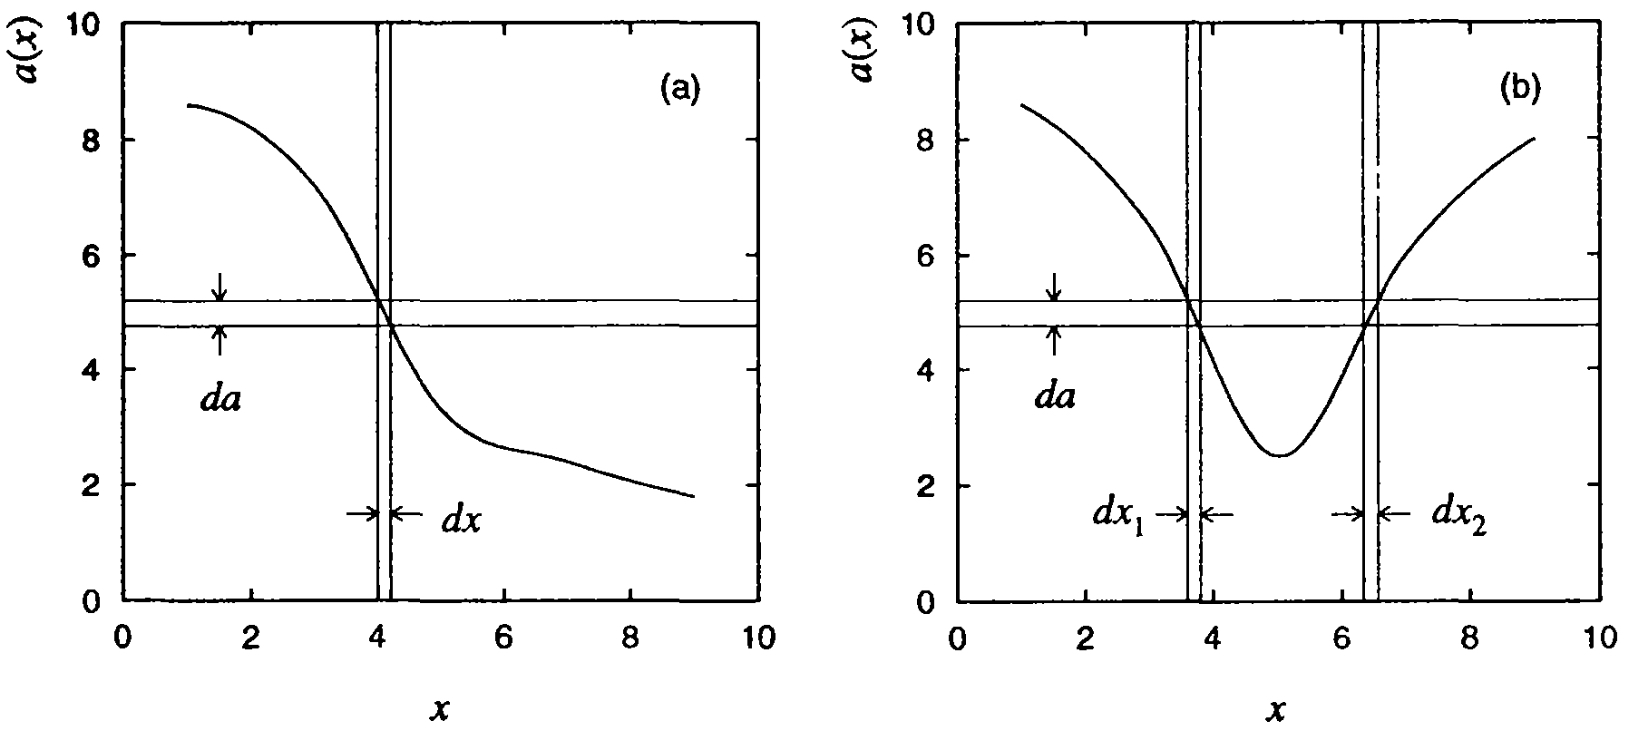
\includegraphics[width=0.65\textwidth,keepaspectratio]{RVfunc}
	\label{fig:RVfunc}
\end{figure}
%Distribuzione di probabilit\'a di $a(X)$ funzione di variabile casuale X con PDF $f(x)$:
\begin{align*}
%&g(a)=f(x(a))|\TDy{a}{x}|\tag*{g(a)\,da=f(x)\,dx}\\
&g(a)\,da=|\int_{x(a)}^{x(a+da)}f(x')\,dx'|=\int_{x(a)}^{x(a)+|\TDy{a}{x}|da}f(x')\,dx'\\
&\Rightarrow g(a)=f(x(a))|\TDy{a}{x}|\\
&g(a')d\,a'=\int_{dS=\{a'\leq a(\vec{x})\leq a'+d\,a'\}}f(x_1,\ldots,x_n)d^n\,x\\
&\prob{(y_1,\ldots,y_n)}=\frac{\prob{(x_1,\ldots,x_n)}}{|\left.\frac{\partial(y_1,\ldots,y_n)}{\partial(x_1,\ldots,x_n)}\right|_{x_1,\ldots,x_n=X_1(\vec{y}),\ldots,X_n(\vec{y})}|}\ (g(\vec{a})=f(\vec{x})|\underset{\PDy{\vec{a}}{\vec{x}}}{J}|)
\end{align*}
\end{frame}

\begin{frame}{Somma di RV: Convoluzione e funzione caratteristica}
\begin{block}{Applicazione cambio di variabile}
Applicando regole cambio variabile per $Z=X+Y$ e $Y'=Y$ e marginalizzando su $Y'$ si trova: $f(Z=X+Y)=\intsinf{}f_X(Z-t)f_Y(t)\,dt$
\end{block}
\begin{block}{Antitrasformata di Fourier prodotto delle funzioni caratteristiche}
\begin{align*}
&X=X_1+X_2\\
&M_X(t)=M_{X_1}M_{X_2}
\end{align*}
La funzione caratteristica determina completamente pdf: se $F(X)$ continua, $dF(X)=f(X)dX$ allora $f(X)=\frac{1}{2\pi}\intsinf{}\phi_X(t)\exp{-iXt}\,dt$.
\end{block}
\end{frame}

\section{Funzione caratteristica/generatrice (dei momenti)}

\begin{frame}{Funzione generatrice dei momenti - Funzione caratteristica}
\begin{columns}[T]
	\begin{column}{0.4\textwidth}
		\begin{align*}
		&M_X(t)=\E{[\exp{tX}]}\\
		&\phi_X(t)=\E{[\exp{itX}]}=\int\exp{itx}\,d\mu_X(x)\\
		&\phi(0)=1,\ |\phi(t)|\leq1\\
		&Y=\alpha X+b:\ M_Y=\exp{ibt}M_X(\alpha t)\\
		&\mu_n(x_0)=\E{[\sum_k^n]}\binom{n}{k}(-1)^{n-k}\mu'_kx_0^{n-k}\\
		&E[a(X)]=\intsinf{}a(x)f(x)dx=\intsinf{}ag(a)da
		\end{align*}
%	Non \'e detto che $f(\mu)=\E{[f]}$.
	\end{column}
	\begin{column}{0.6\textwidth}
		\begin{align*}
		&\PDyn{t}{M_X}{n}|_{t=0}=\E{[x^n]}=\mu_n'\\
		&\PDyn{(it)}{\phi_X}{n}|_{t=0}=(-i)^n\E{[x^n]}=\mu_n'\\
		&\phi_X(t)=\E{[\sum_r\frac{(itX)^r}{r!}]}\\
		&=\sum_r\frac{(it)^r}{r!}\E{[X^r]}=\sum_r\frac{(it)^r}{r!}\mu_r'\\
		&\phi_X(t)=1+i\mu t+\frac{1}{2}(\sigma^2+\mu^2)(it)^2
		\end{align*}
	\end{column}
\end{columns}
Determina completamente pdf: se $F(X)$ continua, $dF(X)=f(X)dX$ allora $f(X)=\frac{1}{2\pi}\intsinf{}\phi_X(t)\exp{-iXt}\,dt$
\begin{block}{Levy theorem: if sequenza $\phi_n\to\phi$ allora $X_n\xrightarrow{D}X$}
Per ogni RV con $\mu$ finita $\phi_X(t)\approx1+i\mu t+o(t)$,$\phi_{\frac{1}{n}X}(t)=\phi_X(\frac{t}{n})$, $\phi_{X+Y}(t)=\phi_X(t)\phi_Y(t)$:
$\phi_{\overline{X}_n}(t)=[\phi_X(t)]^n=[1+it\mu+\ldots]^n\to\exp{i\mu t}$
\end{block}
\end{frame}


\begin{frame}{Funzioni caratteristiche}
COwan 157
\end{frame}

\section{Legge grandi Numeri - T limite centrale}

\begin{frame}{Legge grandi numeri}
\begin{itemize}
\item Chebyshev ineq: $\prob{(|X-\mu|\geq k\sigma)}\leq\frac{1}{k^2}$
\item Probability convergence: 	Una sequenza di RV $\{X_n\}\to X$ in probabilit\'a se $\lim_{n\to\infty}\prob{(|X_n-X|)>\epsilon}$=0
\item LLN: $X_1,\ldots,X_n$ iid RV (RV campionata n volte): $\E{X_i}=\mu$, finite variance: $\var{X_i}=\sigma^2$ allora $\prob{(|\overline{X}_n-\mu|>\epsilon)}\leq\frac{\sigma^2}{n\epsilon^2}$, infatti
\begin{align*}
&\var{\overline{X}_n}=\var{\frac{1}{n}(X_1+\ldots+X_n)}\\
&=\frac{1}{n^2}\var{(X_1+\ldots+X_n)}=\frac{n\sigma^2}{n^2}=\frac{\sigma^2}{n}\\
&\prob{(|\overline{X}_n-\mu|>\epsilon)}\leq\frac{\sigma^2}{n\epsilon^2}
\end{align*}
\end{itemize}
\end{frame}

\begin{frame}{LLN: asintoticamente gaussiana - Teorema limite centrale (CLT)}
Se esistono $\mu_1, \mu_2$ finiti vale LLN: $\overline{x}_n-\mu\xrightarrow{P}0$.
\begin{columns}[T]
	\begin{column}{0.5\textwidth}
		\begin{align*}
		&\var{(\overline{x}_n-\mu)}=\var{(\frac{S_N}{N})}\\
		&=\frac{1}{N^2}\var{(S_N)}=\frac{\sigma^2}{N}\\
		&\var{(S_N)}=\sum(\PDy{x_i}{S_N})^2\sigma_i^2
		%&\phi(t)=\phi_{X-\mu}
		\end{align*}
	\end{column}
	\begin{column}{0.5\textwidth}
		\begin{align*}
		&y_N=\sqrt{\frac{N}{\sigma^2}}(\overline{x}-\mu)\\
		&\E{[y_N]}=0,\ \var{[y_N]}=1\\
		&\phi_N=[\phi(\frac{t}{\sigma\sqrt{N}})]^N
		\end{align*}
	\end{column}
\end{columns}
\[\phi(t)=\sum_{m=0}^{\infty}\left.\frac{d^m\phi}{dt^m}\right|_{t=0}\frac{t^m}{m!}=\sum_{m=0}^{\infty}\frac{(it)^m}{m!}\E{(y^m)}\approx1-\frac{t^2}{2N}\sigma^2-\frac{it^3}{3!}\frac{\E{[(x-\mu)^3]}}{n\expy{3/2}}+\ldots\]
\begin{align*}
&\log{\phi_N}=N\log{\phi(\frac{t}{\sigma\sqrt{N}})}\approx N[\frac{it\mu}{\sigma\sqrt{N}}+\frac{(it)^2\sigma^2}{2\sigma N}+o(\frac{t^3}{N\expy{\frac{3}{2}}})]\\
&\log{\phi_N}\to-\frac{t^2}{2}\\
%\text{Per T Levy la pdf \'e:}\\
&\frac{1}{2\pi}\int\exp{-\frac{t^2}{2}}\exp{-itx}d\,t=\frac{1}{2\pi}\int\exp{(t+ix)^2-\frac{x^2}{2}}d\,t=\frac{1\exp{-\frac{x^2}{2}}}{\sqrt{2\pi}}
\end{align*}
\end{frame}

\section{Data analysis}

\begin{frame}{Statistica}
		\begin{block}{Momenti di una statistica S}
	\begin{align*}
	&\E{[(S(\vec{x})-\E{[S]})^l]}
	\end{align*}
\end{block}
\begin{block}{Propagazione errori}
\begin{align*}
&S(\vec{x})\approx y(\vec{\mu})+\left.\sum_i^n\PDy{x_i}{S}\right|_{\vec{\mu}}(x_i-\mu_i)+o(|\vec{x}-\vec{\mu}|)\\
&\var{(S)}=\E{[(S(\vec{x})-\E{[S]})^2]}\approx\sum_{ij}\PDyat{x_i}{S}{\vec{\mu}}\PDyat{x_i}{y}{\vec{\mu}}\cov{x_ix_j}\\
&\cov{x_ix_j}=\E{[(x-\mu_x)(y-\mu_y)]}=\E{[xy]}-\mu_x\mu_y
\end{align*}
\end{block}
\begin{block}{Statistica sufficiente}
Statistica sufficiente $S$ per parametro $\Theta$. Pdf di X data $T(X)$ non dipende da parametro $\theta$: $\prob{(x;S,\theta)}=\prob{(x;S)}$.
Statistica sufficiente minimale
	$S$ sufficiente e esiste una funzione $f$ per ogni $s_i$ con $S=f(s_i)$ e $\dim({S})\leq\dim{(X)}$.
\end{block}
\end{frame}

\begin{frame}{Funzione di Likelihood}
\begin{columns}[T]
\begin{column}{0.5\textwidth}
$L_{x_0}(m)=p(x_0;m)$, se x,y eventi indipendenti: $L_{(x_0,y_0)}(m)=L_{x_0}(m)L_{y_0}(m)$. Definita a meno di costante moltiplicativa ($\log{L}$): invariante per cambiamento di osservabile (funzione solo dei dati)
$L_{f(t_0)}(m)=|J(t_0)|L_{t_0}(m)$
\end{column}
\begin{column}{0.5\textwidth}
\begin{block}{T di Bayes e likelihood}
Prior $p(\theta)$ contiene belief su parametro fino al nostro esperimento:
\begin{align*}
&p(\theta|x_0)=\frac{p(x_0|\theta)p(\theta)}{p(x_0)}\\
&\posterior{}=\frac{\likelihood{}\prior{}}{\int p(x_0|\theta)p(\theta)\,d\theta}
\end{align*}

Posterior ratio (Degree of belief): $\frac{\Pi(\theta_1|x_0)}{\Pi(\theta_2|x_0)}=\frac{L_{x_0}(\theta_2)}{L_{x_0}(\theta_1)}\frac{\Pi(\theta_2)}{\Pi(\theta_1)}$.
\end{block}
\end{column}
\end{columns} 
\begin{columns}[T]
	\begin{column}{0.5\textwidth}
		\begin{block}{Metodo di massima likelihood}
			Ripetendo gli esperimenti la likelihood diventa pi\'u piccata.
		\end{block}
	\end{column}
	\begin{column}{0.5\textwidth}
		\begin{block}{Likelihood di pi\'u misure e statistiche}
	\begin{align*}
	&\prob{(t,\tau)}=\frac{1}{\tau}\exp{-\frac{t}{\tau}}\\
	&L_{(t_1,\ldots,t_n)}(\tau)=\prod_i^n\frac{1}{\tau}\exp{-\frac{t_i}{\tau}}\\
	&=\frac{1}{\tau^n}\exp{-\frac{\sum t_i}{\tau}}=\frac{1}{\tau^n}\exp{-\frac{n\overline{t}}{\tau}}
	\end{align*}
\end{block}
\end{column}
\end{columns}
\end{frame}

\begin{frame}{Esempi di likelihood}

\end{frame}

\begin{frame}{Bayesian inference}
\end{frame}

\begin{frame}{Statistiche sufficienti per il parametro dato. T di Darmois}

\begin{block}{Teorema di fattorizzazione}
Probabilit\'a di osservare $X$ dato $\theta$ \'e probabilit\'a di $S(x)$ dato $\theta$ per funzione sole osservabili: $\prob{(x;\theta)}=\prob{(S(x);\theta)}h(x)$ e $\omega_{\theta}$ non dipende da $\theta$
\end{block}
\begin{block}{Teorema di Darmois: condizione necessaria e sufficiente per esistenza statistica sufficiente}
Esiste S tale che $\dim{(S)}<\dim{(X)}$ iff
\begin{align*}
&p(\vec{x}|\theta)=\Exp{[\sum_i^n\alpha_i(\vec{x})a_i(\theta)+\beta(\vec{x})+\gamma(\theta)}\\
&S_j=\sum_i\alpha_j(x_i)
\end{align*}
Esiste statistica suff. iff: supporto pdf non dipende da parametro e appartiene alla famiglia esponenziale.
\end{block}
\end{frame}

\section{Stima puntuale}

\section{Stima intervallare}

\begin{frame}[fragile]{Bayesian credibility Interval}
\begin{block}{Credibility (della posterior)}
	\begin{align*}
	&\cred{(x)}=\int_{\mu\in\inf(x)}\Pi(\mu|x)\,d\mu=\int_{\mu\inf(x)}\frac{\prob{(x|\mu)}\prob{(\mu)}}{\int\,d\mu}\,d\mu>\cl{}\\
	&
	\end{align*}
\end{block}
\end{frame}

\section{Test d'ipotesi}

\begin{frame}{Ipotesi semplice. UMP test: Lemma NP.}
RV $\vec{X}$: pdf $f_N(\vec{X}|\theta)$, lo spazio dei parametri \'e $\theta_0,\theta_1$. Cerco la regione $S_0$ regione critica che massimizza power $1-\beta$ (dato $\alpha=\int_{w_{\alpha}}f_N(\vec{X}|\theta_0)\,dX=\alpha$):
\begin{align*}
&\int_{w_{\alpha}}f_N(\vec{X}|\theta_1)\,dX=1-\beta=\int_{w_{\alpha}}\frac{f_N(\vec{X}|\theta_1)}{f_N(\vec{X}|\theta_0)}f_N(\vec{X}|\theta_0)\,dX=\E_{w_{\alpha}}{[\frac{f_N(\vec{X}|\theta_1)}{f_N(\vec{X}|\theta_0)}]}\\
&\Rightarrow l_N(\vec{X},\theta_0,\theta_1)=\frac{f_N(\vec{X}|\theta_1)}{f_N(\vec{X}|\theta_0)}\geq c_{\alpha}: H_1\ (\leq c_{\alpha}: H_0)
\end{align*}
Per ogni test alternativo $T'$ prendo $\alpha'\leq\alpha_{NP}$ allora $\beta'\geq\beta_{NP}$ ($\pow'\leq\pow_{NP}$, probabilit\'a errore tipo II \'e maggiore), dimostro $\beta'-\beta\geq0$ cio\'e $\prob{(\overline{C}'|H_1)}-\prob{(\overline{C}|H_1)}$:
\begin{align*}
&\prob{(C|H_1)}-\prob{(C'|H_1)}=\prob{(C\cap|H_1)}+\prob{(C\cap\overline{C}'|H_1)}-\prob{(C\cap C'|H_1)}-\prob{(C'\cap\overline{C}|H_1)}=\prob{(C\cap\overline{C}'|H_1)}-\prob{(C'\cap\overline{C}|H_1)}\\
&\prob{(C\cap C'|H_1)}=\int_{C\cap C'}\prob_1{(x)}\,dx\geq\int_{C\cap \overline{C}'}\frac{\prob_0{(x)}}{q}\,dx=\frac{1}{q}\prob{(C\cap\overline{C}'|H_0)}
\end{align*}
\end{frame}

\begin{frame}{Ipotesi composte}
For exponential family exists UMP one-sided ($H_0: \theta=\theta_0$, $H_1: \theta>\theta_0$)
\end{frame}

\begin{frame}{LMP test}
Se ho bisogno di massima sensibilit\'a vicino alla soglia: $1-\beta$ grande nelle vicinanze di 0: $H_0$: $\theta=\theta_0$, $H_1$: $\theta=\theta_0+\Delta$, quindi $\ln{L(\vec{X},\theta_1)}\approx\ln{L(\vec{X},\theta_0)}+\Delta\PDy{\theta}{\ln{L}}|_{\theta_0}$.
Applico NP a $H_0$ vs $H_1$:
\begin{equation*}
\ln{L(\vec{X},\theta_1)}-\ln{L(\vec{X},\theta_0)}\gtrless c_{\alpha} \Rightarrow \PDy{\theta}{\ln{L}}\gtrless q_{\alpha}
\end{equation*}
\begin{columns}[T]
	\begin{column}{0.4\textwidth}
		\begin{align*}
		&H_0: \theta=\theta_0\\
		&H_1: \theta=\theta_0+\Delta
		\end{align*}
	\end{column}
	\begin{column}{0.6\textwidth}
		\begin{align*}
		&\PDy{\theta}{\log{L}}\gtrless k_{\alpha}\gtrless\lambda_{\alpha}\sqrt{NI}\\
		&\E{[\PDy{\theta}{\log{L}}|_{\theta_0}]}=0,\ \E{[(\PDy{\theta}{\log{L}}|_{\theta_0})^2]}=NI
		\end{align*}
	\end{column}
\end{columns}
\end{frame}

\begin{frame}{LR test}
James pg 287
\end{frame}

\section{Compiti}\linkdest{compiti}

\begin{wordonframe}{Combinazione p-value per 10 osservabili indipendenti (16/07/18)}
	Fit di massima likelihood per le 10 osservabili (binned) basandosi su teoria: istogrammi suff. popolati per GOF test di Pearson con 30 dof (31 bins?)
	\begin{table}[h!]
		\centering
		\begin{tabular}{||cccccc||} 
			$\chi^2(/30?)$&38.33&40.87&30.70&36.91&39.97\\
			&36.97&20.48&32.34&41.32&41.41\\
			$P(\chi^2_{30}<x)$&0.859&0.911&0.570&0.820&0.894\\
			&0.822&0.096&0.648&0.918&0.920\\
		\end{tabular}
	\end{table}
	Impressione che ci siano troppi valori alti del $\chi^2$: come risolvere il dubbio in maniera rigorosa?
	\begin{itemize}
	\item \keyword{additivit\'a del $\chi^2$}: somma quadrati di RV normali standard.
			Sommando $\chi^2$ in tab si ottiene RV con pdf $\chi^2_{300}$ approssimabile con gaussiana con $\sigma=\sqrt{2N}\approx24.5$.
			$\sum_i\chi^2_i=359.3$, siamo a $1.21\sigma$
	\item KS test: campione di 10 valori in accordo con pdf $\chi^2_{30}$ (cumulante $\prob{(\chi^2_{30}<x)}$ in tabella). Calcolo $F_n(x_{k-1})-F_n(x_k)$ e $F_n(x_k)-F_n(x_k)$:  $|0-0.096|$, $|0.1-0.57|$, $|0.2-0.648|$, $|0.3-0.82|$, $|0.4-0.822|$, $|0.5-0.859|$, $|0.6-0.894|$, $|0.7-0.914|$, $|0.8-0.918|$, $|0.9-0.926|$; $\Delta=0.52$??
	\item Combinazione diretta p-values: $p_i=1-\prob{(\chi^2_{30}<x)}$, \keyword{pdf somma log p-values} $-2\log{(\prod^Np_i)}$ ha pdf $\chi^2_{2N}$
	\item Test binned: hist of p-values (3-4) e considero LR con pdf uniforme (\keyword{pdf p-value}) e quindi usarlo per test basato su pdf asintotica (esatta, calcolandola)
	\item Considerare max(min) dei p-values e usare pdf $x_M$ per test
	\item Test della mediana
	\item Test basato su propriet\'a pdf $\chi^2_{30}$: test varianza $2N$; test secondo momento attorno a media nominale 30.
\end{itemize}
\end{wordonframe}

\begin{wordonframe}{Stimatori, confidence/credible interval per parametro m di pdf uniforme da misura della mediana(16/07/18)}
\begin{columns}[T]\begin{column}{0.5\textwidth}
x RV $U(0,m)$; $2k+1=3$ misura la mediana $x_2=3.4$
\begin{block}{MLE estimator, bias, incertezza statistica}
\begin{align*}
&\prob{(\mu=x_2)}=6\frac{\mu}{m^2}(1-\frac{\mu}{m})\\
&\hat{\mu}_{MLE}=3/2\mu\\
&\E{[\hat{m}]}=\frac{3}{2}\E{[\mu]}\frac{3}{2}\int_0^{m}\mu\prob{(\mu)}\,d\mu\\
&=\frac{3}{4}m\\
&\hat{m}'=\frac{4}{3}\hat{m}=2\mu\\
&\var{[\hat{m}]}=\sigma^2_{\hat{m}}=\frac{9}{4}\var{\mu}=\frac{9}{4}\sigma_{\mu}^2\\
&\var{[\hat{m}']}=\sigma^2_{\hat{m}'}=4\var{\mu}=4\sigma_{\mu}^2\\
&\sigma^2_{\mu}=\exv{\mu^2}-\exv{\mu}^2=\frac{m^2}{20}
\end{align*}
Le varianze sono funzione del valore di m: le stimo usando $\hat{m}$
\end{block}
\end{column}\begin{column}{0.5\textwidth}
Likelihood pdf uniforme: \begin{equation*}L_x(m)=\left\{\begin{array}{c}
0\ m<x\\
1/m\ m\geq x\\
\end{array}\right.
\end{equation*}
Determinazione $p(\mu=x_2)$ dove $\mu$ pu\'o essere vista come seconda misura pi\'u grande o mediana; per $2k+1$ misure
\begin{align*}
&\prob{(\mu;m)}=\prob{(\mu)}F(\mu)^k[1-F(\mu)]^k\\
&(2k+1)\binom{2k}{k}\\
&\prob{(\mu;m)}=\frac{1}{m}(\frac{\mu}{m})^k(1-\frac{\mu}{m})^k\frac{(2k+1)!}{k!k!1!}
\end{align*}
\vspace{5cm}
\begin{block}{\keyword{Stima bayesiana di m}}
Assumo prior uniforme in $\log{m}$: $\prob{(m)}\propto\frac{1}{m}$, \keyword{posterior} $\pi(m)\propto L(\mu|m)\prob{(m)}=\frac{6\mu}{m^3}-\frac{6\mu^2}{m^4}$ ($\prob{(H)}=\frac{\prob{(E|H)\prob{(H)}}}{\prob{(E)}}$): la posterior va normalizzata tra $[\mu,+\infty]$ (likelihood nulla  in $[0,\mu]$), $\pi(m)=\frac{3\mu^2}{m^3}-\frac{3\mu^3}{m^4}$, il massimo fornisci una stima bayesiana di m: $\hat{m}=\frac{4}{3}\mu$.
\end{block}
\end{column}\end{columns}
\end{wordonframe}

\begin{wordonframe}{Stimatori, confidence/credible interval per parametro m di pdf uniforme da misura della mediana(16/07/18)}
	\begin{columns}[T]\begin{column}{0.5\textwidth}
			\begin{block}{MLE estimator, bias, incertezza statistica}
				\begin{align*}
				&\var{[\hat{m}']}=\sigma^2_{\hat{m}'}=4\var{\mu}=4\sigma_{\mu}^2\\
				&\sigma^2_{\mu}=\exv{\mu^2}-\exv{\mu}^2=\frac{m^2}{20}
				\end{align*}
				Le varianze sono funzione del valore di m: le stimo usando $\hat{m}$
			\end{block}
		\end{column}\begin{column}{0.5\textwidth}
			\begin{block}{\keyword{Stima bayesiana di m}}
				Assumo prior uniforme in $\log{m}$: $\prob{(m)}\propto\frac{1}{m}$, \keyword{posterior} $\pi(m)\propto L(\mu|m)\prob{(m)}=\frac{6\mu}{m^3}-\frac{6\mu^2}{m^4}$ ($\prob{(H)}=\frac{\prob{(E|H)\prob{(H)}}}{\prob{(E)}}$): la posterior va normalizzata tra $[\mu,+\infty]$ (likelihood nulla  in $[0,\mu]$), $\pi(m)=\frac{3\mu^2}{m^3}-\frac{3\mu^3}{m^4}$, il massimo fornisci una stima bayesiana di m: $\hat{m}=\frac{4}{3}\mu$.
			\end{block}
	\end{column}\end{columns}
\end{wordonframe}

\begin{wordonframe}{Stimatori, confidence/credible interval per parametro m di pdf uniforme da misura della mediana(16/07/18)}
	\begin{block}{Limite superiore/bilaterale}
		\keyword{Limite superiore per m di $U(0,m)$ da mediana campionaria}: $\int_{\mu}^m6\frac{\tilde{\mu}}{m^2}(1-\frac{\tilde{\mu}}{m})\,d\tilde{\mu}=\cl=0.9$, con $y=\frac{\mu}{m}$ si risolve $F(\mu)=y^2(3-2y)=1-\cl$ ha soluzione $y=0.1958$ quindi $m<\frac{\mu}{0.1958}$.
		\keyword{Limite bilaterali simmetrici per m da mediana campionaria}: $F(\mu)=y^2(3-2y)=(1-\cl)/2$ $y_+=0.13535$, $\int_{\mu}^m6\frac{\tilde{\mu}}{m^2}(1-\frac{\tilde{\mu}}{m})\,d\tilde{\mu}=(1-\cl)/2$ quindi $F(\mu)=y^2(3-2y)=(1+\cl)/2$ e $y_-=0.8647$: Limiti bilaterali con $\cl=0.9$ sono $\frac{\mu}{0.8647}<m<\frac{\mu}{0.13535}$
	\end{block}
	\begin{block}{Limiti credibilit\'a Bayesiana}
		prior uniform, $\cred=90\%$. La posterior \'e $\pi(m)=\frac{2\mu}{m^2}-\frac{2\mu^2}{m^3}$ diversa da zero in $[\mu,+\infty]$ e la cumulante $F(m)=\int_{\mu}^m\pi(\tilde{m})\,d\tilde{m}=1+\mu(\frac{\mu}{m^2}-\frac{2}{m})$:
		\begin{align*}
		&F(m_{min})=\frac{1-\cl}{2}\\
		&F(m_{max})=\frac{1+\cl}{2}\\
		&\frac{\mu}{1-\sqrt{(1-\cl)/2}}<m<\frac{\mu}{1-\sqrt{(1+\cl)/2}}
		\end{align*}
		dove ho scelto le soluzioni maggiori di $\mu$, per il limite superiore si ha $m<66.26$.
	\end{block}
	\begin{block}{Limiti confidenza al $90\%\cl$ a la FC}
		Imponiamo il LR-ordering e coverage $90\%$
		\begin{equation*}
		\lambda\propto\mu\prob{(\mu;m)}=6\frac{\mu^2}{m^2}(1-\frac{\mu}{m})
		\end{equation*}
		LR \'e unimodale: un intervallo con $\lambda(m_1)=\lambda(m_2)$, mentre il coverage richiede $\int_{m_1}^{m_2}\prob{(\mu;m)}\,d\mu=\cl$ da cui si ottiene il sistema di equazioni
		\begin{align*}
		&y_2^3-y_1^3=\cl\\
		&y_2^2-y_1^2=\cl\\
		&y_1=\frac{m_1}{m},\ y_1=\frac{m_1}{m}\\
		&\frac{\mu}{0.96804}<m<\frac{\mu}{0.192606}
		\end{align*}
	\end{block}
	\begin{block}{$2k+1$ misure: propriet\'a statistica mediana per costruzione estimatori}
		pdf per mediana campionaria
		\begin{equation*}
		\prob{(\mu;m)}=\frac{1}{m}(\frac{\mu}{m})^k(1-\frac{\mu}{m})^k\frac{(2k+1)!}{k!k!1!}
		\end{equation*}
		\keyword{stimatore massima likelihood}:
		\begin{align*}
		&\log{L(m)}=\log{\frac{1}{m}}+k\log{\frac{\tilde{m}}{m}}+k\log{(1-\frac{\tilde{m}}{m})}+\const{}\\
		&\TDy{m}{\log{L}}=0 \Rightarrow \hat{m}=\frac{2k+1}{k+1}\tilde{m}
		\end{align*}
		Bias estimatore:
		\begin{align*}
		&\E{[\hat{m}]}=\frac{2k+1}{k+1}\E{[\tilde{m}]}\\
		&\E{[\tilde{m}]}=\int_0^m\tilde{m}\prob{(\tilde{m};m)}\,d\tilde{m}\\
		&=\frac{(2k+1)!}{k!k!1!}m\int_0^1x^{k+1}(1-x)^k\,dx\ (x=\frac{\tilde{m}}{m})\\
		&\E{[\tilde{m}]}=\frac{(2k+1)!}{k!k!1!}m\frac{\Gamma(k+1)\Gamma(k+2)}{\Gamma(2k+3)}=\frac{m}{2}\ (\Gamma(k+1)=k!)\\
		&\E{[\hat{m}]}=\frac{2k+1}{2(k+1)}m\\
		&b=m-\frac{2k+1}{2(k+1)}=\frac{1}{2(k+1)}m\to0
		\end{align*}
		Varianza
		\begin{align*}
		&\E{[\tilde{m}^2]}=\frac{(2k+1)!}{k!k!1!}m^2\int_0^1x^{k+2}(1-x)^k\,dx\\
		&=\frac{(2k+1)!}{k!k!1!}m^2\frac{\Gamma(k+1)\Gamma(k+3)}{\Gamma(2k+4)}\\
		&=\frac{(k+1)(k+1)}{(2k+3)(2k+2)}m^2\\
		&\var{[\tilde{m}]}=\E{[\tilde{m}^2]}-\E{[\tilde{m}]}^2=m^2\frac{1}{4(2k+3)}\\
		&\var{[\hat{m}]}=(\frac{2k+1}{k+1})^2\var{[\tilde{m}]}\to0
		\end{align*}
		\keyword{Efficienza estimatore mediana campionaria per pdf uniforme}: non si pu\'o usare MVB come riferimento assoluto dato che per pdf uniforme $I_F$ non \'e proporzionale al numero di misure; efficienza relativa rispetto a stimatore ricavato da statistica suff. $x_M$ $\var{[x_M]}=frac{m^2}{k^2}$: il MLE ricavato da mediana \'e meno efficiente ed efficienza relativa va a 0.
	\end{block}
\end{wordonframe}

\begin{wordonframe}{Stime limite superiore dati da pdf uniforme (Compito 09/11/18)}
\begin{block}{\keyword{pdf di $X_{(2)}$ per N estrazioni da pdf uniforme}}
\begin{align*}
&\prob{X_{(k)}<x}=\sum_{i=k}^nc(n,i)F(x)^i[1-F(x)]^{n-i}\\
&\PDof{p}\sum_{i=k}^nc(n,i)p^{i}[1-p]^{n-i}=nC(n-1,k-1)p\expy{k-1}(1-p)\expy{k-1}\\
&\prob{(X_{(k)})}=nC(n-1,k-1)f(x)F(x)\expy{k-1}(1-F(x))\expy{k-1}\\
&\prob{(x_2;m)}=N(N-1)\frac{1}{m^N}x_2\expy{N-2}(m-x_2)
\end{align*}
\end{block}
\begin{block}{Efficienza stimatore di m da statistica $x_2$}
Massimizzando $L(m)$ per m si ha $\hat{m}=\frac{N}{N-1}x_2$, si corregge per il bias $\E{[\hat{m}]}-m=-\frac{1}{N+1}m$ definendo $\hat{m}'=\frac{N+1}{N}\hat{m}=\frac{N+1}{N-1}x_2$; per calcolare la varianza
\begin{align*}
\var{[\hat{m}']}=\E{\hat{m}'^2}-\E{[\hat{m}']}^2\\
\E{[\hat{m}'^2]}=\frac{(N+1)^2}{(N-1)^2}\E{[x_2^2]}=\frac{2}{(N-1)(N+2)}m^2
\end{align*}
\end{block}
\begin{block}{Efficienza stimatore di m da statistica $x_M$}
\keyword{pdf di $x_M$} \'e $\frac{N}{m}(\frac{x_M}{m})^{N-1}$: stima di \keyword{massima likelihood di m da statistica $x_M$}: $\hat{m}=x_M$; stimatore unbiased $\hat{m}'=\frac{N+1}{N}\hat{m}$.
La varianza di $\hat{m}'$ \'e
\begin{align*}
&\E{[\hat{m}'^2]}-\E{\hat{m'}}^2=\frac{(N+1)^2}{N^2}\frac{N}{N+2}m^2-m^2=\frac{1}{N(N+2)}m^2
\end{align*}
\end{block}
\begin{block}{Confronto efficienza stimatore da $x_2$ vs $x_M$}
L'\keyword{efficienza relativa di due stimatori} si ottiene:
\begin{equation*}
\epsilon_r=\frac{\var{[\hat{m'}_{M}]}}{\var{[\hat{m'}_{x_2}]}}
\end{equation*}
\end{block}
\begin{block}{\keyword{Combinazione likelihood 2 misure di $x_2$}}
Calcolare MLE massimizzando likelihood combinata:
\begin{align*}
&L(m_1,m_2;x_2'x_2'')=N^2(N-1)^2\frac{1}{m^{2N}}{x_2'}^{N-1}{x_2''}^{N-2}(m-x_2')(m-x_2'')\\
&2(N-1)m^2+(x_2'+x_2'')(2N-1)m-2N(x_2'x_2'')=0\\
&\hat{m}_{\pm}=\frac{(x_2'+x_2'')(2N-1)\pm\sqrt{(x_2'+x_2'')^2(2N-1)^2-16N(N-1)x_2'x_2''}}{4(N-1)}
\end{align*}
quale soluzione \'e nella regione in cui la likelihood \'e diversa da zero? Asintoticamente $\hat{m}=\max{(x_2',x_2'')}$ (Assumo $x_2''>x_2'$)
\end{block}
\begin{block}{\keyword{Test bilaterale di ipotesi composte: dati da pdf uniforme con $m_1\neq m_2$?}}
Likelihood ratio test:
\begin{equation*}
\lambda(x_1',x_2'')=-2\log{\frac{\sup_m{p(x_2',x_2'';m)}}{\sup_{m_1,m_2}{p(x_2',x_2'';m_1,m_2)}}}
\end{equation*}
\keyword{chiarire cosa significa massimizzare likleihood combinata per pi\'u parametri o uno!}
\begin{align*}
&\hat{m}=f(N)x_2\Rightarrow p(x_2',\hat{m})=G(N)/x_2',\ p(x_2'',\hat{m})=G(N)/x_2''\\
&\sup_{m_1,m_2}{p(x_2',x_2'';m_1,m_2)}\propto\frac{1}{x_2'x_2''},\ p(x_2',x_2'';m)\propto(m-x_2')(m-x_2'')(x_2'x_2'')^{N-2}\\
&??\sup_{m}p(x_2',x_2'';m)\propto x_2''(x_2''-x_2')(x_2'x_2'')^{N-2}
\end{align*}
\keyword{Likelihood ratio monotona (asintoticamente): statistica $t(x_2',x_2'')=x_2''/x_2'$}: il test LR \'e della forma $x_2''/x_2'>q_{\alpha}$
\keyword{Monotone LR in statistic $T(x)$} and \keyword{Karlin-Rubin theorem}
\end{block}
\end{wordonframe}

\begin{wordonframe}{Stima di tempo medio tra eventi di onde gravitazionali}
Conteggi generati da eventi casuali statisticamente indipendenti: distribuzione del tempo tra due eventi (Poissoniana con $n\approx1$) esponenziale $\prob{(t;\tau)}=\frac{1}{\tau}\exp{-\frac{t}{\tau}}$. Il massimo della likelihood ci fornisce stimatore $\hat{t}=t_m=\SI{39}{\day}$ quindi ha la stessa distribuzione esponenziale dei tempi t: $\E{[\hat{\tau}]}=\tau$, $\var{[\tau]}=\tau^2$ quindi $\hat{\tau}=\SI{0.107+-107}{\year}$.
Il \keyword{MLE trasforma in modo banale sotto cambio di variabile}: $\hat{\lambda}=\hat{\frac{1}{\tau}}=\SI{9.3}{\counts\per\year}$; usando formula per propagazione errori si ha
\begin{equation*}
\sigma(\lambda)=\sqrt{\var{[\hat{\lambda}]}}\approx\frac{1}{\tau^2}\sqrt{\var{[\tau]}}
\end{equation*}
Tuttavia l'\keyword{approssimazione quasi lineare del cambio di variabile} \'e una pessima approssimazione sull'ampio intervallo di incertezze della variabile originale.
La distribuzione di $\hat{\lambda}=\frac{1}{\hat{\tau}}$ \'e:
\begin{equation*}
\prob{(\hat{\lambda},\lambda)}=\prob{(\hat{\tau}(\hat{\lambda});\lambda=\frac{1}{\tau})}|\TDy{\hat{\lambda}}{\hat{\tau}(=\frac{1}{\hat{\lambda}})}|
\end{equation*}
Momenti di ordine $>0$ non esistono: $\var{[\lambda]}=\infty$.
\keyword{bande di confidenza per pdf esponenziale}
Stima intervallare di $\lambda=\frac{1}{\tau}$ e $\prob{(t;\lambda)}=\lambda\exp{-\lambda t}$. \keyword{probability ordering}: pdf \'e monotona decrescente in t quindi p-ordering equivale a $o(t)=-t$, $t\leq t_{max}(\lambda)$
\begin{align*}
&\int_0^{t_{max}}\lambda\exp{-\lambda t}\,dt=\cl{}\\
&t_{max}(\lambda)=-\frac{\log{(1-\cl{})}}{\lambda}
\end{align*}
$t_{max}(\lambda)$ decrescente in $\lambda$, da $t<t_{max}(\lambda)$ si vede che \keyword{la banda di confidenza \'e della forma $t<t_{max}(\lambda)$ porta a limite $\lambda\leq\lambda_{max}$} (limite superiore); l'inversione porta a $\lambda_{max}=-\frac{\log{(1-\cl{})}}{t_m}$.
Per ottenere limite inferiore occorre ordinamento $o(t)=t$:
\begin{equation*}
\int_{t_{min}}^{\infty}\lambda\exp{-\lambda t}\,dt=\cl{}\Rightarrow t_{min}(\lambda)=-\frac{\log{(\cl{})}}{\lambda}
\end{equation*}
banda della forma $t\geq t_{min}(\lambda)$ porta, essendo $t_{min}(\lambda)$ decrescente il $\lambda$, a limite inferiore $\lambda\geq\lambda_{min}=-\frac{\log{(\cl{})}}{t_m}$. Limite inferiore a un fenomeno nuovo!

LR-ordering:
\begin{equation*}
\lr{}=\frac{\prob{(t;\lambda)}}{\sup_{\lambda}\prob{(t;\lambda)}}=\lambda t\exp{-\lambda t}
\end{equation*}
fissato $\lambda$ ha singolo massimo in t e monotona da ambo i lati: usando $o(t)=\lr{(t)}$ ottengo intervallo $[t_{min},t_{max}]$.

\keyword{prior impropria}: in mancanza di una scala definita utilizzo prior uniforme in $[0,\infty]$ (non normalizabile). Devo normalizare la \keyword{posterior}:
\begin{align*}
&\pi(\lambda|t_m)\propto \lambda\exp{-t_m\lambda}=L_{t_m}(\lambda)\\
&\pi(\lambda|t_m)=t_m^2\lambda\exp{-t_m\lambda}
\end{align*}
quindi \keyword{limite bayesiano inferiore}
\begin{equation*}
\int_{\lambda_{min}}^{\infty}t_m^2\lambda\exp{-t_m\lambda}\,d\lambda=\cl{}
\end{equation*}

\keyword{limite bayesiano bilaterale simmetrico}:
\begin{align*}
&\int_0^{\lambda_{min}}t_m^2\lambda\exp{-t_m\lambda}\,d\lambda=\frac{1-\cl}{2}\\
&\int_{\lambda_{max}}^{\infty}t_m^2\lambda\exp{-t_m\lambda}\,d\lambda=\frac{1-\cl}{2}
\end{align*}

\keyword{limite bayesiano utilizzando posterior ordering}:
\begin{align*}
&\exp{-t_m\lambda_{min}}(t_m\lambda_{min}+1)-\exp{-t_m\lambda_{max}}(t_m\lambda_{max}+1)=\cl\\
&\lambda_{min}\exp{-t_m\lambda_{min}}-\lambda_{max}\exp{-t_m\lambda_{max}}=0
\end{align*}


\end{wordonframe}

\begin{wordonframe}{math basic}
\begin{block}{Soluzione equazione di secondo grado}
\begin{align*}
&4a(ax^2+bx+c)=0\\
&4a^2x^2+4abx+4ac+b^2-b^2=0\\
&(2ax+b)^2=b^2-4ac
\end{align*}
\end{block}

\end{wordonframe}
